\chapter[Revisão teórica]{Revisão teórica} \label{cap:revisao}
    Colocar texto aqui 
    
    \section{Sistema Multirrobô} \label{sec:mrs}
        Colocar texto aqui
    
        \subsection{Taxonomias} \label{subsec:taxonomias_mrs}
    
    \section{Alocação de Tarefa em Sistema Multirrobô} \label{sec:mrta}
        Um dos problemas mais desafiadores em aplicações multirrobô leva o nome \textit{alocação de tarefa}, na língua inglesa, \textit{Multi-Robot Task Allocation}(MRTA). Problemas dessa natureza buscam como solução atribuir otimamente um conjunto de robôs para um conjunto de tarefas de maneira que o desempenho geral de um sistema sujeito a um conjunto de limitações seja otimizado.
        
        \textcolor{red}{falar sobre o conteúdo desta seção}
        
        
        \subsection{Definição Formal} \label{subsec:mrta_formal}
            \citeonline{ref:zlot2006auction} define o problema de alocação de tarefa em um sistema multirrobô conforme abaixo.
            
            \begin{definicao} \label{def:mrta}
                (\textit{Alocação de Tarefa em um Sistema Multirrobô})
                Sejam dados um conjunto $T$, um conjunto $R$ e uma função de custo para cada subconjunto de robots $r \in R$ que especifique o custo de performance para cada subconjunto de tarefas, $c_r : 2^T \to \mathbb{R}_+\cup\{\infty\}$: procure a alocação $A^* \in R^T$ que minimiza a função objetivo global $C : R^T \to \mathbb{R}_+\cup\{\infty\}$.
            \end{definicao}
        
            Note que para que um algoritmo consiga encontrar uma solução ótima para este problema, é necessário levar em consideração todo o espaço de alocação $R^T$, cujo tamanho aumenta exponencialmente em função do número de tarefas e robôs no sistema. 
            
            %Muitas arquiteturas simplificam este problema possa ter uma solução viável em tempo real.
            
            
    
        \subsection{Taxonomia} \label{subsec:taxonomia_mrta}
            \citeonline{ref:gerkey2004taxonomy} sugeriram uma taxonomia de três eixos independente do domínio para a classificação de problemas de alocação de tarefas em sistemas multirrobôs. 
            
            O primeiro eixo determina o \textit{tipo dos robôs} que compõem o problema. Os tipos de robôs possíveis são: \textit{ST} (acrônimo para \textit{Single-Task}) ou \textit{MT} (acrônimo para \textit{Multi-Task}). Problemas que envolvem robôs que só podem executar uma tarefa por vez são compostos por robôs do tipo \textit{ST}. Entretanto, se houver pelo menos um robô capaz de executar mais de uma tarefa simultaneamente, então esse problema é composto por robôs do tipo \textit{MT}. 
            
            O segundo eixo da taxonomia determina o \textit{tipo das tarefas} que compõem o problema. Nesse caso, são possíveis os tipos: \textit{ST} (acrônimo para \textit{Single-Robot}) ou \textit{MR} (acrônimo para \textit{Multi-Robot}). Problemas cujo tipo das tarefas é \textit{SR}, diz-se que todas as tarefas envolvidas só podem ser executadas por um robô. Porém, quando o tipo das tarefas envolvidas é \textit{MR}, diz-se que existe tarefas que podem ser executadas por mais de um robô.
            
            O terceiro eixo, por sua vez, determina o \textit{tipo da alocação} do problema, o qual pode assumir os valores: \textit{IA} (acrônimo para \textit{Instantaneous Assignment}) ou \textit{TA} (acrônimo para \textit{Time-extended Assignment}). O primeiro caso, \textit{IA}, diz repeito à problemas MRTA onde as alocações das tarefas para os robôs são realizadas instantaneamente, sem levar em consideração o estado futuro do sistema. Por outro lado, em problemas cujo tipo de alocação é \textit{TA}, além de conhecido o estado atual de cada rôbo e do ambiente, também é conhecido o conjunto de tarefas que precisarão ser alocadas no futuro. Neste último caso, diversas tarefas são alocadas para um robô, o qual deve executar cada alocação conforme seu agendamento. De acordo com \cite{ref:bastos2008utility}, quando o tipo de alocação do problema MRTA é \textit{IA}, o número de robôs é superior ao número de tarefas alocadas e quando \textit{TA}, o oposto acontece. Isso se deve ao fato de que, em problemas MRTA cujo tipo de alocação é \textit{IA}, o número de robôs no sistema é capaz de suprir a taxa de tarefas a serem atribuídas, de modo que é muito provável que haverão robôs ociosos no sistema; enquanto, naqueles cujo tipo de alocação é \textit{TA}, o número de robôs que compõem o sistema não é suficiente para atender a taxa de tarefas a serem alocadas no sistema.
            
            \begin{figure}[htb]
                \centering
                % Graphic for TeX using PGF
% Title: ../figures/taxonomia_mrta.dia
% Creator: Dia v0.97.2
% CreationDate: Tue Oct 17 17:33:09 2017
% For: adrianohrl
% \usepackage{tikz}
% The following commands are not supported in PSTricks at present
% We define them conditionally, so when they are implemented,
% this pgf file will use them.
\ifx\du\undefined
  \newlength{\du}
\fi
\setlength{\du}{15\unitlength}
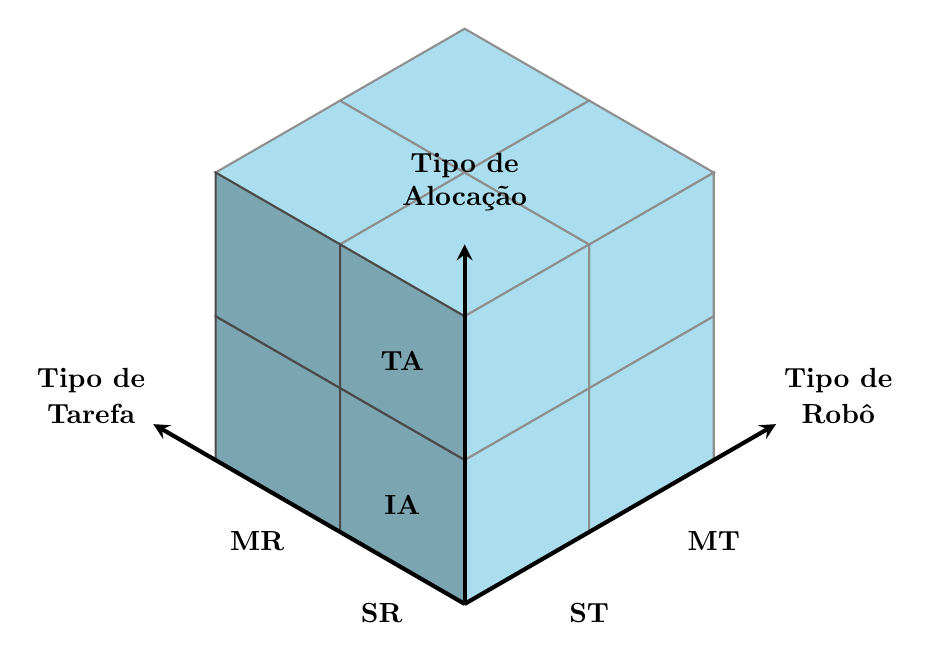
\begin{tikzpicture}
\pgftransformxscale{1.000000}
\pgftransformyscale{-1.000000}
\definecolor{dialinecolor}{rgb}{0.000000, 0.000000, 0.000000}
\pgfsetstrokecolor{dialinecolor}
\definecolor{dialinecolor}{rgb}{1.000000, 1.000000, 1.000000}
\pgfsetfillcolor{dialinecolor}
\pgfsetlinewidth{0.050000\du}
\pgfsetdash{}{0pt}
\pgfsetdash{}{0pt}
\pgfsetmiterjoin
\pgfsetbuttcap
\definecolor{dialinecolor}{rgb}{0.666667, 0.870588, 0.937255}
\pgfsetfillcolor{dialinecolor}
\fill (-5.500000\du,-10.392300\du)--(-2.500000\du,-8.660250\du)--(0.500000\du,-10.392300\du)--(-2.500000\du,-12.124400\du)--cycle;
\definecolor{dialinecolor}{rgb}{0.556863, 0.556863, 0.556863}
\pgfsetstrokecolor{dialinecolor}
\draw (-5.500000\du,-10.392300\du)--(-2.500000\du,-8.660250\du)--(0.500000\du,-10.392300\du)--(-2.500000\du,-12.124400\du)--cycle;
\pgfsetlinewidth{0.050000\du}
\pgfsetdash{}{0pt}
\pgfsetdash{}{0pt}
\pgfsetmiterjoin
\pgfsetbuttcap
\definecolor{dialinecolor}{rgb}{0.666667, 0.870588, 0.937255}
\pgfsetfillcolor{dialinecolor}
\fill (-2.500000\du,-12.124400\du)--(0.500000\du,-10.392300\du)--(3.500000\du,-12.124400\du)--(0.500000\du,-13.856400\du)--cycle;
\definecolor{dialinecolor}{rgb}{0.556863, 0.556863, 0.556863}
\pgfsetstrokecolor{dialinecolor}
\draw (-2.500000\du,-12.124400\du)--(0.500000\du,-10.392300\du)--(3.500000\du,-12.124400\du)--(0.500000\du,-13.856400\du)--cycle;
\pgfsetlinewidth{0.050000\du}
\pgfsetdash{}{0pt}
\pgfsetdash{}{0pt}
\pgfsetmiterjoin
\pgfsetbuttcap
\definecolor{dialinecolor}{rgb}{0.666667, 0.870588, 0.937255}
\pgfsetfillcolor{dialinecolor}
\fill (3.500000\du,-8.660250\du)--(3.500000\du,-5.196150\du)--(6.500000\du,-6.928200\du)--(6.500000\du,-10.392300\du)--cycle;
\definecolor{dialinecolor}{rgb}{0.556863, 0.556863, 0.556863}
\pgfsetstrokecolor{dialinecolor}
\draw (3.500000\du,-8.660250\du)--(3.500000\du,-5.196150\du)--(6.500000\du,-6.928200\du)--(6.500000\du,-10.392300\du)--cycle;
\pgfsetlinewidth{0.050000\du}
\pgfsetdash{}{0pt}
\pgfsetdash{}{0pt}
\pgfsetmiterjoin
\pgfsetbuttcap
\definecolor{dialinecolor}{rgb}{0.666667, 0.870588, 0.937255}
\pgfsetfillcolor{dialinecolor}
\fill (-2.500000\du,-8.660250\du)--(0.500000\du,-6.928200\du)--(3.500000\du,-8.660250\du)--(0.500000\du,-10.392300\du)--cycle;
\definecolor{dialinecolor}{rgb}{0.556863, 0.556863, 0.556863}
\pgfsetstrokecolor{dialinecolor}
\draw (-2.500000\du,-8.660250\du)--(0.500000\du,-6.928200\du)--(3.500000\du,-8.660250\du)--(0.500000\du,-10.392300\du)--cycle;
\pgfsetlinewidth{0.050000\du}
\pgfsetdash{}{0pt}
\pgfsetdash{}{0pt}
\pgfsetmiterjoin
\pgfsetbuttcap
\definecolor{dialinecolor}{rgb}{0.666667, 0.870588, 0.937255}
\pgfsetfillcolor{dialinecolor}
\fill (0.500000\du,-10.392300\du)--(3.500000\du,-8.660250\du)--(6.500000\du,-10.392300\du)--(3.500000\du,-12.124400\du)--cycle;
\definecolor{dialinecolor}{rgb}{0.556863, 0.556863, 0.556863}
\pgfsetstrokecolor{dialinecolor}
\draw (0.500000\du,-10.392300\du)--(3.500000\du,-8.660250\du)--(6.500000\du,-10.392300\du)--(3.500000\du,-12.124400\du)--cycle;
\pgfsetlinewidth{0.050000\du}
\pgfsetdash{}{0pt}
\pgfsetdash{}{0pt}
\pgfsetmiterjoin
\pgfsetbuttcap
\definecolor{dialinecolor}{rgb}{0.666667, 0.870588, 0.937255}
\pgfsetfillcolor{dialinecolor}
\fill (0.500000\du,-6.928200\du)--(0.500000\du,-3.464100\du)--(3.500000\du,-5.196150\du)--(3.500000\du,-8.660250\du)--cycle;
\definecolor{dialinecolor}{rgb}{0.556863, 0.556863, 0.556863}
\pgfsetstrokecolor{dialinecolor}
\draw (0.500000\du,-6.928200\du)--(0.500000\du,-3.464100\du)--(3.500000\du,-5.196150\du)--(3.500000\du,-8.660250\du)--cycle;
\pgfsetlinewidth{0.050000\du}
\pgfsetdash{}{0pt}
\pgfsetdash{}{0pt}
\pgfsetmiterjoin
\pgfsetbuttcap
\definecolor{dialinecolor}{rgb}{0.666667, 0.870588, 0.937255}
\pgfsetfillcolor{dialinecolor}
\fill (0.500000\du,-3.464100\du)--(0.500000\du,0.000000\du)--(3.500000\du,-1.732050\du)--(3.500000\du,-5.196150\du)--cycle;
\definecolor{dialinecolor}{rgb}{0.556863, 0.556863, 0.556863}
\pgfsetstrokecolor{dialinecolor}
\draw (0.500000\du,-3.464100\du)--(0.500000\du,0.000000\du)--(3.500000\du,-1.732050\du)--(3.500000\du,-5.196150\du)--cycle;
\pgfsetlinewidth{0.050000\du}
\pgfsetdash{}{0pt}
\pgfsetdash{}{0pt}
\pgfsetmiterjoin
\pgfsetbuttcap
\definecolor{dialinecolor}{rgb}{0.666667, 0.870588, 0.937255}
\pgfsetfillcolor{dialinecolor}
\fill (3.500000\du,-5.196150\du)--(3.500000\du,-1.732050\du)--(6.500000\du,-3.464100\du)--(6.500000\du,-6.928200\du)--cycle;
\definecolor{dialinecolor}{rgb}{0.556863, 0.556863, 0.556863}
\pgfsetstrokecolor{dialinecolor}
\draw (3.500000\du,-5.196150\du)--(3.500000\du,-1.732050\du)--(6.500000\du,-3.464100\du)--(6.500000\du,-6.928200\du)--cycle;
\pgfsetlinewidth{0.050000\du}
\pgfsetdash{}{0pt}
\pgfsetdash{}{0pt}
\pgfsetmiterjoin
\pgfsetbuttcap
\definecolor{dialinecolor}{rgb}{0.486275, 0.647059, 0.698039}
\pgfsetfillcolor{dialinecolor}
\fill (-2.500000\du,-8.660250\du)--(-2.500000\du,-5.196150\du)--(-5.500000\du,-6.928200\du)--(-5.500000\du,-10.392300\du)--cycle;
\definecolor{dialinecolor}{rgb}{0.290196, 0.290196, 0.290196}
\pgfsetstrokecolor{dialinecolor}
\draw (-2.500000\du,-8.660250\du)--(-2.500000\du,-5.196150\du)--(-5.500000\du,-6.928200\du)--(-5.500000\du,-10.392300\du)--cycle;
\pgfsetlinewidth{0.050000\du}
\pgfsetdash{}{0pt}
\pgfsetdash{}{0pt}
\pgfsetmiterjoin
\pgfsetbuttcap
\definecolor{dialinecolor}{rgb}{0.486275, 0.647059, 0.698039}
\pgfsetfillcolor{dialinecolor}
\fill (0.500000\du,-6.928200\du)--(0.500000\du,-3.464100\du)--(-2.500000\du,-5.196150\du)--(-2.500000\du,-8.660250\du)--cycle;
\definecolor{dialinecolor}{rgb}{0.290196, 0.290196, 0.290196}
\pgfsetstrokecolor{dialinecolor}
\draw (0.500000\du,-6.928200\du)--(0.500000\du,-3.464100\du)--(-2.500000\du,-5.196150\du)--(-2.500000\du,-8.660250\du)--cycle;
\pgfsetlinewidth{0.050000\du}
\pgfsetdash{}{0pt}
\pgfsetdash{}{0pt}
\pgfsetmiterjoin
\pgfsetbuttcap
\definecolor{dialinecolor}{rgb}{0.486275, 0.647059, 0.698039}
\pgfsetfillcolor{dialinecolor}
\fill (-2.500000\du,-5.196150\du)--(-2.500000\du,-1.732050\du)--(-5.500000\du,-3.464100\du)--(-5.500000\du,-6.928200\du)--cycle;
\definecolor{dialinecolor}{rgb}{0.290196, 0.290196, 0.290196}
\pgfsetstrokecolor{dialinecolor}
\draw (-2.500000\du,-5.196150\du)--(-2.500000\du,-1.732050\du)--(-5.500000\du,-3.464100\du)--(-5.500000\du,-6.928200\du)--cycle;
\pgfsetlinewidth{0.050000\du}
\pgfsetdash{}{0pt}
\pgfsetdash{}{0pt}
\pgfsetmiterjoin
\pgfsetbuttcap
\definecolor{dialinecolor}{rgb}{0.486275, 0.647059, 0.698039}
\pgfsetfillcolor{dialinecolor}
\fill (0.500000\du,-3.464100\du)--(0.500000\du,0.000000\du)--(-2.500000\du,-1.732050\du)--(-2.500000\du,-5.196150\du)--cycle;
\definecolor{dialinecolor}{rgb}{0.290196, 0.290196, 0.290196}
\pgfsetstrokecolor{dialinecolor}
\draw (0.500000\du,-3.464100\du)--(0.500000\du,0.000000\du)--(-2.500000\du,-1.732050\du)--(-2.500000\du,-5.196150\du)--cycle;
% setfont left to latex
\definecolor{dialinecolor}{rgb}{0.000000, 0.000000, 0.000000}
\pgfsetstrokecolor{dialinecolor}
\node at (-8.500000\du,-5.374900\du){\textbf{Tipo de}};
% setfont left to latex
\definecolor{dialinecolor}{rgb}{0.000000, 0.000000, 0.000000}
\pgfsetstrokecolor{dialinecolor}
\node at (-8.500000\du,-4.574900\du){\textbf{Tarefa}};
% setfont left to latex
\definecolor{dialinecolor}{rgb}{0.000000, 0.000000, 0.000000}
\pgfsetstrokecolor{dialinecolor}
\node at (0.500000\du,-10.571050\du){\textbf{Tipo de}};
% setfont left to latex
\definecolor{dialinecolor}{rgb}{0.000000, 0.000000, 0.000000}
\pgfsetstrokecolor{dialinecolor}
\node at (0.500000\du,-9.771050\du){\textbf{Alocação}};
% setfont left to latex
\definecolor{dialinecolor}{rgb}{0.000000, 0.000000, 0.000000}
\pgfsetstrokecolor{dialinecolor}
\node at (9.500000\du,-5.374900\du){\textbf{Tipo de}};
% setfont left to latex
\definecolor{dialinecolor}{rgb}{0.000000, 0.000000, 0.000000}
\pgfsetstrokecolor{dialinecolor}
\node at (9.500000\du,-4.574900\du){\textbf{Robô}};
\pgfsetlinewidth{0.100000\du}
\pgfsetdash{}{0pt}
\pgfsetdash{}{0pt}
\pgfsetbuttcap
{
\definecolor{dialinecolor}{rgb}{0.000000, 0.000000, 0.000000}
\pgfsetfillcolor{dialinecolor}
% was here!!!
\pgfsetarrowsstart{stealth}
\definecolor{dialinecolor}{rgb}{0.000000, 0.000000, 0.000000}
\pgfsetstrokecolor{dialinecolor}
\draw (8.000000\du,-4.330130\du)--(0.500000\du,0.000000\du);
}
\pgfsetlinewidth{0.100000\du}
\pgfsetdash{}{0pt}
\pgfsetdash{}{0pt}
\pgfsetbuttcap
{
\definecolor{dialinecolor}{rgb}{0.000000, 0.000000, 0.000000}
\pgfsetfillcolor{dialinecolor}
% was here!!!
\pgfsetarrowsstart{stealth}
\definecolor{dialinecolor}{rgb}{0.000000, 0.000000, 0.000000}
\pgfsetstrokecolor{dialinecolor}
\draw (-7.000000\du,-4.330130\du)--(0.500000\du,0.000000\du);
}
% setfont left to latex
\definecolor{dialinecolor}{rgb}{0.000000, 0.000000, 0.000000}
\pgfsetstrokecolor{dialinecolor}
\node at (-4.500000\du,-1.510800\du){\textbf{MR}};
% setfont left to latex
\definecolor{dialinecolor}{rgb}{0.000000, 0.000000, 0.000000}
\pgfsetstrokecolor{dialinecolor}
\node at (-1.500000\du,0.221250\du){\textbf{SR}};
% setfont left to latex
\definecolor{dialinecolor}{rgb}{0.000000, 0.000000, 0.000000}
\pgfsetstrokecolor{dialinecolor}
\node at (3.500000\du,0.221250\du){\textbf{ST}};
% setfont left to latex
\definecolor{dialinecolor}{rgb}{0.000000, 0.000000, 0.000000}
\pgfsetstrokecolor{dialinecolor}
\node at (6.500000\du,-1.510800\du){\textbf{MT}};
% setfont left to latex
\definecolor{dialinecolor}{rgb}{0.000000, 0.000000, 0.000000}
\pgfsetstrokecolor{dialinecolor}
\node at (-1.000000\du,-5.840930\du){\textbf{TA}};
% setfont left to latex
\definecolor{dialinecolor}{rgb}{0.000000, 0.000000, 0.000000}
\pgfsetstrokecolor{dialinecolor}
\node at (-1.000000\du,-2.376830\du){\textbf{IA}};
\pgfsetlinewidth{0.100000\du}
\pgfsetdash{}{0pt}
\pgfsetdash{}{0pt}
\pgfsetbuttcap
{
\definecolor{dialinecolor}{rgb}{0.000000, 0.000000, 0.000000}
\pgfsetfillcolor{dialinecolor}
% was here!!!
\pgfsetarrowsstart{stealth}
\definecolor{dialinecolor}{rgb}{0.000000, 0.000000, 0.000000}
\pgfsetstrokecolor{dialinecolor}
\draw (0.500000\du,-8.660250\du)--(0.500000\du,0.000000\du);
}
\end{tikzpicture}

                \caption[Representação visual da taxonomia de três eixos]{Representação visual da taxonomia de três eixos sugerida por \citeonline{ref:gerkey2004taxonomy}.} \label{fig:taxomia_mrta}
            \end{figure}
            
            É visto na Figura \ref{fig:taxomia_mrta} uma representação gráfica da taxonomia de \cite{ref:gerkey2004taxonomy} para a classificação de problemas MRTA (\textit{Multi-Robot Task Allocation}), onde pode-se notar que existem oito classes de problemas MRTA bem definidos.
            
        \subsubsection{Arquitetura MRTA} \label{subsec:arquiteturas_mrta}
            Possue a função de solucionar o problema de alocação de tarefas em um dado sistema multirrobô.
            
            Basicamente existem duas formas de implementação de uma arquitetura iterativas e instantâneas. As aproximações iterativas apresentam uma dinâmica progressiva para que ocorra um alocação, enquanto as arquiteturas que esperam uma resposta instantânea dos robôs do sistema ...
        
            \subsection{Arquiteturas baseadas em Comportamento} \label{subsec:arch_comportamento}
            
            \begin{itemize}
                \item \textbf{ALLIANCE}: \cite{ref:parker1998alliance};
                \item \textbf{L-ALLIANCE}: \cite{ref:parker1996lalliance};
                
            \end{itemize}
            
            \subsection{Arquiteturas baseadas em Mercado} \label{subsec:arch_mercado}
    
            \begin{itemize}
                \item \textbf{Murdoch}: \cite{ref:gerkey2002murdoch};
                \item \textbf{M+}: \cite{ref:botelho1999m+};
                
            \end{itemize}
                
    \section{ROS - Robot Operating System} \label{sec:ros}
        Acrônimo para \textit{Robot Operating System} \cite{ref:quigley2009ros}, o ROS é um \textit{framework} para robótica que tem incentivado a comunidade de pesquisadores desta área do conhecimento a trabalhar conjuntamente desde seu lançamento. Ao observar o grande avanço desta ferramenta de comunicação, muitos fabricantes de manipuladores industriais iniciaram a investir em pesquisas para integrar seus robôs com o ROS. 
        
        Uma lacuna que antes existia na nova geração de aplicações robóticas foi preenchida com o lançamento do ROS. Como um fornecedor de serviços de \textit{middleware}, ele (1) simplifica o desenvolvimento de processos, (2) suporta comunicação e interoperabilidade, (3) oferece e facilita serviços frequentemente utilizados em robótica e, ainda, oferece (4) utilização eficiente dos seus recursos disponíveis, (5) abstrações heterogênicas e (6) descoberta e configuração automática de recursos \cite{ref:quigley2009ros}. No intuito de cobrir todas exigências de um \textit{middleware}, ROS 2.0 tenta dar suporte à sistemas embarcados e dispositivos de baixo recurso.
    
        No ROS, projetos atômicos são chamados \textit{pacotes} e podem ser desenvolvido em diversas linguagens de programação. Isso mostra que o ROS é flexível, pois seus usuários podem tirar proveito das vantagens que cada linguagem suportada tem, sejam elas eficiência em tempo de execução, confiabilidade, recursos, síntaxe, semântica, suporte ou documentação existente. Atualmente, as linguagens de programação suportadas são C++, Python e Lisp. As linguagens Java e Lua ainda estão em fase de desenvolvimento.
        
        Projetos de robótica possuem rotinas que poderia ser reutilizadas em outros projetos. Por esta razão, ROS é também modular, pois pacotes configuráveis existentes podem ser combinados para realizar uma aplicação especifica de robótica. Várias bibliotecas externas já foram adaptadas para serem usadas no ROS: aruco\footnote{\url{http://wiki.ros.org/ar_sys}}, gmapping\footnote{\url{http://wiki.ros.org/gmapping}}, interfaces de programação para aplicações de robôs\footnote{\url{http://wiki.ros.org/Robots}}, sensores\footnote{\url{http://wiki.ros.org/Sensors}} e simuladores\footnote{\url{http://wiki.ros.org/gazebo}}, planejadores\footnote{\url{http://kcl-planning.github.io/ROSPlan/}}, reconhecimento de voz\footnote{\url{http://wiki.ros.org/Sensors\#Audio_.2BAC8_Speech_Recognition}}, entre outros. Isso evidencia que os usuários de ROS podem focar no desenvolvimento de pesquisa de sua área e contribuir da melhor forma com essa comunidade.
        
        Enfim, ROS disponibiliza diversas ferramentas para auxiliar no desenvolvimento de projetos e, também, verificar o funcionamento de aplicação. Suas ferramentas típicas são: \textit{get} e \textit{set} de parâmetros de configuração, vizualização da topologia de conexão \textit{peer-to-peer}, medição de utilização de banda, gráficos dos dados de mensagem e outras mais. É altamente recomendado o uso dessas ferramentas para garantir a estabilidade e confiança dos pacotes desenvolvidos, que normalmente têm alta complexidade.
        
        Esta seção apresenta conceitos básicos para entender o funcionamento desta \textit{framework}. Em seguida, são expostas as regras de nomenclatura dos recursos do ROS. E, então, é brevemente dado suporte sobre a construção de aplicações gráficas integradas com o ROS.
        
        \subsection{Conceitos Básicos} \label{subsec:ros_conceitos}
            Sua concepção foi fundada sobre conceitos divididos em três níveis: (1) Sistema de Arquivos do ROS, (2) Grafo de Computação do ROS e (3) Comunidade do ROS. A seguir será explicado cada um desses níveis, cada um com seu respectivo conjunto de conceitos. Além disso, também serão detalhados os dois tipos de nomes definidos no ROS: nomes de recursos de pacote e nomes de recursos de grafo.
            
            \subsubsection{Sistema de Arquivos do ROS} \label{subsubsec:ros_arquivos}
                Os conceitos envolvidos no nível do \textit{Sistema de Arquivos do ROS} se referem aos arquivos armazenados em disco. São eles:
                
                \begin{itemize}
                    \item \textbf{Pacotes}: em inglês \textit{Packages}, é uma forma atômica de organização de criação e lançamento de \textit{software} no ROS. Um pacote contém definições de processos (nós), de dependência de bibliotecas, de tipos de mensagens, ações e serviços, de estruturas de dados e, por fim, de configuração. 
                    
                    \item \textbf{Meta-Pacotes}: em inglês \textit{Metapackages}, é um tipo especial de pacote que tem por objetivo agrupar pacotes relacionados.
                    
                    \item \textbf{Manifestos de Pacote}: em inglês \textit{Package Manifests}, arquivo nomeado \textit{package.xml} contido na raíz de cada pacote. Seu papel é fornecer meta-informações sobre seu pacote: nome, versão, descrição, informações de licença, dependências, entre outras. 
                    
                    \item \textbf{Tipos de Mensagem}: em inglês \textit{Message Types}, arquivos de extensão \textit{.msg}, localizados dentro da pasta \textit{msg} de um dado pacote. Seu conteúdo define a estrutura de dados de uma mensagem que poderá ser enviado pelo ROS.
                    
                    \item \textbf{Tipos de Serviço}: em inglês \textit{Service Types}, arquivos de extensão \textit{.srv}, localizados dentro da pasta \textit{srv} de um dado pacote. Seu conteúdo define a estrutura de dados das mensagens de requisito e resposta de um serviço, as quais poderão ser enviadas pelo ROS.
                \end{itemize}
            
            \subsubsection{Grafo de Computação do ROS} \label{subsubsec:ros_grafo}
                O \textit{Grafo de Computação do ROS} é uma rede ponto-a-ponto de processos que processam dados conjuntamente. Os conceitos presentes neste nível são:
                
                \begin{itemize}
                    \item \textbf{Nós}: em inglês \textit{Nodes}, são processos computacionais que são executados para desempenhar o controle de atuadores, realizar leitura e filtragem de sinais sensoriais ou implementar algoritmos avançados de planejamento e tomada de decisão. É desejável que os nós sejam desenvolvidos da forma mais genérica possível, para sua reutilização em outros projetos. Cada linguagem de programação suportada encapsula as funcionalidades do ROS em uma biblioteca. Para a escrita de um nó na linguagem C++, é utilizada a biblioteca do pacote \textit{roscpp}\footnote{\url{http://wiki.ros.org/roscpp}} e, para escrever um nó em Python, é utilizada a biblioteca contida no pacote \textit{rospy}\footnote{\url{http://wiki.ros.org/rospy}};
                    
                    \item \textbf{Nó Mestre}: em inglês \textit{Master}, fornece cadastro e pesquisa de nome no Grafo de Computação do ROS, ou seja, este nó é responsável por garantir a comunicação entre os nós. Sem a sua execução, não existe comunicação entre os nós.
                    
                    \item \textbf{Servidor de Parâmetros}: em inglês \textit{Parameter Server}, parte do Nó Mestre que centraliza a consulta e o armazenamento de dados indexados por uma cadeia de caracteres.
                    
                    \item \textbf{Mensagens}: em inglês \textit{Messages}, a comunicação entre os nós no ROS consiste no transporte de mensagens, as quais são estruturas de dados que possuem campos tipados. Os campos de uma mensagem podem ser do tipo primitivo (booleano, inteiro, ponto flutuante, caracter, enumerado, cadeia de caracteres), aninhar outras mensagens ou vetores desses tipos. 
                    
                    \item \textbf{Tópicos}: em inglês \textit{Topics}, são canais que ligam os nós para o transporte de mensagens utilizando a semântica de comunicação \textit{publish/subscribe}. Assim, nós que enviam mensagens para o sistema, as publica no tópico e nós recebem as mensagens ao assinar o tópico. Cada tópico possui um tipo, o que lhe permite transportar apenas este tipo de mensagem. Como característica da sua semântica, vários nós podem publicar e se inscrever no mesmo tópico. E um nó pode publicar e se inscrever em vários tópicos;
                    
                    \item \textbf{Serviços}: em inglês \textit{Services}, é um sistema de comunicação no ROS que obedece a semântica \textit{request/reply}. Neste caso, um nó cliente solicita um serviço através de um pedido para um nó servidor que, por sua vez, retorna uma resposta ao nó cliente ao finalizar o serviço prestado.
                    
                    \item \textbf{Bolsas}: do inglês \textit{Bags}, são arquivos de extensão \textit{.bag} que contêm dados de mensagens do ROS.
                \end{itemize}
                
                A Figura \ref{fig:ros_conceitos_basicos} ilustra os tipos básicos de comunicação entre nós no ROS. Nessa figura, nós são representados por elipses, tópicos por retângulos, conexões entre nó e tópico por setas de linha contínua e invocações de serviço por setas de linha tracejada. Verifica-se assim que o \textit{Nó 1} publica no \textit{Tópico} e o \textit{Nó 2} o subscreve. Além disso, o \textit{Nó 1} é servidor do \textit{Serviço} e o \textit{Nó 2} é seu cliente.
                
                \begin{figure}
                    \centering
                    % Graphic for TeX using PGF
% Title: ../figures/ros/ros_conceitos_basicos.dia
% Creator: Dia v0.97.2
% CreationDate: Sat Nov 11 16:55:11 2017
% For: adrianohrl
% \usepackage{tikz}
% The following commands are not supported in PSTricks at present
% We define them conditionally, so when they are implemented,
% this pgf file will use them.
\ifx\du\undefined
  \newlength{\du}
\fi
\setlength{\du}{15\unitlength}
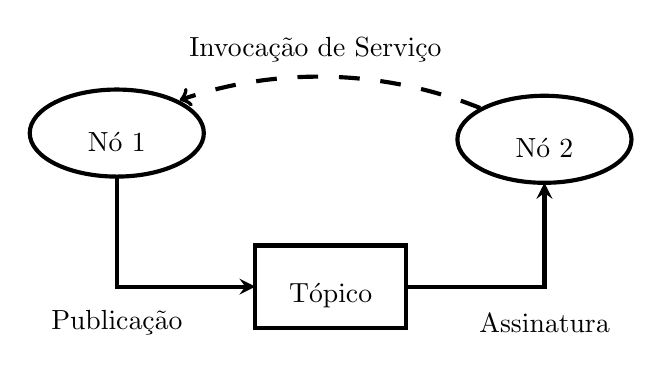
\begin{tikzpicture}
\pgftransformxscale{1.000000}
\pgftransformyscale{-1.000000}
\definecolor{dialinecolor}{rgb}{0.000000, 0.000000, 0.000000}
\pgfsetstrokecolor{dialinecolor}
\definecolor{dialinecolor}{rgb}{1.000000, 1.000000, 1.000000}
\pgfsetfillcolor{dialinecolor}
\definecolor{dialinecolor}{rgb}{1.000000, 1.000000, 1.000000}
\pgfsetfillcolor{dialinecolor}
\pgfpathellipse{\pgfpoint{14.648284\du}{13.550742\du}}{\pgfpoint{2.096884\du}{0\du}}{\pgfpoint{0\du}{1.048442\du}}
\pgfusepath{fill}
\pgfsetlinewidth{0.100000\du}
\pgfsetdash{}{0pt}
\pgfsetdash{}{0pt}
\pgfsetmiterjoin
\definecolor{dialinecolor}{rgb}{0.000000, 0.000000, 0.000000}
\pgfsetstrokecolor{dialinecolor}
\pgfpathellipse{\pgfpoint{14.648284\du}{13.550742\du}}{\pgfpoint{2.096884\du}{0\du}}{\pgfpoint{0\du}{1.048442\du}}
\pgfusepath{stroke}
% setfont left to latex
\definecolor{dialinecolor}{rgb}{0.000000, 0.000000, 0.000000}
\pgfsetstrokecolor{dialinecolor}
\node at (14.648284\du,13.764770\du){Nó 1};
\definecolor{dialinecolor}{rgb}{1.000000, 1.000000, 1.000000}
\pgfsetfillcolor{dialinecolor}
\pgfpathellipse{\pgfpoint{24.950384\du}{13.700742\du}}{\pgfpoint{2.096884\du}{0\du}}{\pgfpoint{0\du}{1.048442\du}}
\pgfusepath{fill}
\pgfsetlinewidth{0.100000\du}
\pgfsetdash{}{0pt}
\pgfsetdash{}{0pt}
\pgfsetmiterjoin
\definecolor{dialinecolor}{rgb}{0.000000, 0.000000, 0.000000}
\pgfsetstrokecolor{dialinecolor}
\pgfpathellipse{\pgfpoint{24.950384\du}{13.700742\du}}{\pgfpoint{2.096884\du}{0\du}}{\pgfpoint{0\du}{1.048442\du}}
\pgfusepath{stroke}
% setfont left to latex
\definecolor{dialinecolor}{rgb}{0.000000, 0.000000, 0.000000}
\pgfsetstrokecolor{dialinecolor}
\node at (24.950384\du,13.914770\du){Nó 2};
\definecolor{dialinecolor}{rgb}{1.000000, 1.000000, 1.000000}
\pgfsetfillcolor{dialinecolor}
\fill (17.986900\du,16.259000\du)--(17.986900\du,18.240944\du)--(21.611900\du,18.240944\du)--(21.611900\du,16.259000\du)--cycle;
\pgfsetlinewidth{0.100000\du}
\pgfsetdash{}{0pt}
\pgfsetdash{}{0pt}
\pgfsetmiterjoin
\definecolor{dialinecolor}{rgb}{0.000000, 0.000000, 0.000000}
\pgfsetstrokecolor{dialinecolor}
\draw (17.986900\du,16.259000\du)--(17.986900\du,18.240944\du)--(21.611900\du,18.240944\du)--(21.611900\du,16.259000\du)--cycle;
% setfont left to latex
\definecolor{dialinecolor}{rgb}{0.000000, 0.000000, 0.000000}
\pgfsetstrokecolor{dialinecolor}
\node at (19.799400\du,17.464000\du){Tópico};
\pgfsetlinewidth{0.100000\du}
\pgfsetdash{{1.000000\du}{1.000000\du}}{0\du}
\pgfsetdash{{0.500000\du}{0.500000\du}}{0\du}
\pgfsetbuttcap
{
\definecolor{dialinecolor}{rgb}{0.000000, 0.000000, 0.000000}
\pgfsetfillcolor{dialinecolor}
% was here!!!
\pgfsetarrowsend{to}
\definecolor{dialinecolor}{rgb}{0.000000, 0.000000, 0.000000}
\pgfsetstrokecolor{dialinecolor}
\pgfpathmoveto{\pgfpoint{23.403259\du}{12.947952\du}}
\pgfpatharc{292}{251}{10.338566\du and 10.338566\du}
\pgfusepath{stroke}
}
\pgfsetlinewidth{0.100000\du}
\pgfsetdash{}{0pt}
\pgfsetdash{}{0pt}
\pgfsetmiterjoin
\pgfsetbuttcap
{
\definecolor{dialinecolor}{rgb}{0.000000, 0.000000, 0.000000}
\pgfsetfillcolor{dialinecolor}
% was here!!!
\pgfsetarrowsend{stealth}
{\pgfsetcornersarced{\pgfpoint{0.000000\du}{0.000000\du}}\definecolor{dialinecolor}{rgb}{0.000000, 0.000000, 0.000000}
\pgfsetstrokecolor{dialinecolor}
\draw (21.611900\du,17.249972\du)--(24.950384\du,17.249972\du)--(24.950384\du,14.749184\du);
}}
% setfont left to latex
\definecolor{dialinecolor}{rgb}{0.000000, 0.000000, 0.000000}
\pgfsetstrokecolor{dialinecolor}
\node at (24.950400\du,18.120050\du){Assinatura};
% setfont left to latex
\definecolor{dialinecolor}{rgb}{0.000000, 0.000000, 0.000000}
\pgfsetstrokecolor{dialinecolor}
\node at (14.648400\du,18.120050\du){Publicação};
% setfont left to latex
\definecolor{dialinecolor}{rgb}{0.000000, 0.000000, 0.000000}
\pgfsetstrokecolor{dialinecolor}
\node at (19.433900\du,11.522450\du){Invocação de Serviço};
\pgfsetlinewidth{0.100000\du}
\pgfsetdash{}{0pt}
\pgfsetdash{}{0pt}
\pgfsetmiterjoin
\pgfsetbuttcap
{
\definecolor{dialinecolor}{rgb}{0.000000, 0.000000, 0.000000}
\pgfsetfillcolor{dialinecolor}
% was here!!!
\pgfsetarrowsend{stealth}
{\pgfsetcornersarced{\pgfpoint{0.000000\du}{0.000000\du}}\definecolor{dialinecolor}{rgb}{0.000000, 0.000000, 0.000000}
\pgfsetstrokecolor{dialinecolor}
\draw (14.648284\du,14.599184\du)--(14.648284\du,17.249972\du)--(17.986900\du,17.249972\du);
}}
\end{tikzpicture}

                    \caption{Conceitos básicos de comunicação do ROS.}
                    \label{fig:ros_conceitos_basicos}
                \end{figure}
                
                Nós que publicam mensagens em um tópico só estão interessados em disponibilizar a informação, não importando com quem irá utilizá-lo. Da mesma forma, um nó que assina um tópico está apenas interessado em receber a informação disponível no tópica sem se importar com sua fonte. Deste modo, é aconselhado utilizar esse tipo de comunicação na troca de dados de fluxo contínuo, por exemplo, dados de sensores e sinais de atuação e controle.
                
                Uma invocação de serviço é equivalente a chamada remota de um procedimento. Quando um cliente de serviço solicita um pedido ao seu servidor, ambos ficam aguardando o procedimento finalizar. Com isso, é recomendado o uso desse tipo de comunicação em casos onde o serviço prestado é rápido, como alterações do estado de alguma variável interna.
                
                Vale salientar que muitas mensagens e serviços já foram padronizadas em pacotes do ROS\footnote{\url{http://wiki.ros.org/common_msgs}}.
            
            \subsubsection{Comunidade do ROS} \label{subsubsec:ros_comunidade}
                De modo que comunidades separadas possam trocar código fonte e conhecimento, vários recursos foram criados na \textit{Comunidade do ROS}. Tais como:
                
                \begin{itemize}
                    \item \textbf{Distribuições}: agrupa coleções de pacotes versionados para facilitar a instalação do ROS. Além disso, é mantido uma versão consistente de cada conjunto de pacotes relacionados.
                    
                    \item \textbf{Repositórios}: uma rede federada de repositórios de código permite que instituições diferentes possam desenvolver e lançar componentes de \textit{software} para seus próprios robôs.
                    
                    \item \textbf{ROS Wiki\footnote{\url{http://wiki.ros.org}}}: é o principal fórum para informações de documentação sobre o ROS. Qualquer pessoa pode solicitar uma conta para contribuir com sua própria documentação, ou ainda fornecer correções e atualizações, bem como, escrever tutoriais.
                    
                    \item \textbf{Listas de endereços eletrônicos}: é o meio de comunicação primário entre os usuários de ROS para perguntar sobre questões de \textit{software} do ROS e para receber notificações de novas atualizações.
                    
                    \item \textbf{ROS Answers\footnote{\url{https://answers.ros.org/questions/}}}: é uma página \textit{web} de perguntas e respostas diretamente relacionada ao ROS.
                    
                    \item \textbf{Blog\footnote{\url{http://www.ros.org/news/}}}: providencia notícias regularmente com fotos e vídeos.
                \end{itemize}
            
            \subsubsection{Nome de Recurso de Grafo} \label{subsubsec:ros_nomes_grafo}
            
                Os recursos de grafo presentes no ROS são: nós, parâmetros, tópicos e serviços. Com o uso adequado da sintaxe de nomes, é possível obter encapsulamento desses recursos através do mecanismo que os nomeia, pois ele gera uma estrutura hierárquica de nomes. Em outras palavras, cada recurso no ROS possui um \textit{namespace} que pode ser compartilhado com vários outros recursos. Normalmente, recursos podem criar outros recursos dentro do seu próprio \textit{namespace} e acessar recursos que estão dentro ou acima dele. Contudo, recursos em camadas inferiores podem ser acessados através da integração de código em \textit{namespaces} superiores. Abaixo, seguem exemplos de nomes de recurso no ROS.
                
                \begin{itemize}
                    \item /
                    
                    \item /rqt\_mrta
                    
                    \item /lro/p3dx/pose
                    
                    \item /lro/amigobot/pose
                    
                    \item /lro/alliance
                \end{itemize}
                
                O primeiro exemplo mostra o \textit{namespace} global (/). Todos os recursos com seu respectivo \textit{namespace} estão sob ele. O exemplo seguinte mostra um recurso denominado \textit{rqt\_mrta} cujo \textit{namespace} se encontra no nível mais alto. Em seguida, verifica-se três exemplos de recursos que estão sob o \textit{namespace lro}. Entretanto, os recursos mostrados nos terceiro e quarto exemplos ainda estão sob um outro \textit{namespace}, \textit{p3dx} e \textit{amigobot}, respectivamente. Note que neste caso, o nome de ambos recursos são iguais (\textit{pose}), porém eles são diferenciados pelos seus \textit{namespaces} (\textit{/lro/p3dx} e \textit{/lro/amigobot}, respectivamente). Por último, é dado o recurso cujo nome é \textit{alliance} que se encontra sob o \textit{namespace /lro}. 
                
                Existem quatro tipos de resolução de nomes de recursos no ROS: \textit{base}, \textit{relativa}, \textit{global} e \textit{privada}.
                
                \begin{itemize}
                    \item base
                    
                    \item relativa/nome
                    
                    \item /global/nome
                    
                    \item \textasciitilde privada/nome
                \end{itemize}
                
                Nomes são resolvidos relativamente, então recursos não necessitam estar cientes de qual \textit{namespace} eles se encontram. Isso simplifica a programação como nós que trabalham em conjunto podem ser escritos como se eles estivessem todos no nível de \textit{namespace} mais alto.
                
                \begin{table}[hbt]
                    \centering
                    \caption{Exemplos de resolução de nomes no ROS}
                    \label{tab:ros_nomes}
                    \begin{tabular}{llll}
                        \textbf{Nó} & \textbf{Relativa} &  \textbf{Global} & \textbf{Privada} \\
                        /no & img$\to$/no/img & /img$\to$/img & \textasciitilde img$\to$/no/img \\
                        /no & img/raw$\to$/no/img/raw & /img/raw$\to$/img/raw & \textasciitilde img/raw$\to$/no/img/raw \\
                        /ns/no & img$\to$/ns/no/img & /img$\to$/img & \textasciitilde img$\to$/ns/no/img
                    \end{tabular}
                \end{table}
                
                Esses conceitos possuem extrema importância em sistemas multirrobô, principalmente naqueles cuja frota de robôs é homogênea. Neste último caso, a partir de replicação das configurações de um robô, todo o sistema pode ser iniciado, variando apenas o \textit{namespace} de cada robô do sistema.
            
            \subsubsection{Nome de Recursos de Pacote} \label{subsubsec:ros_nomes_pacotes}
            
        \subsection{Interface Gráfica de Usuário do ROS}
            Além de ferramentas disponíveis em terminal via comando de linha, o ROS também disponibiliza ferramentas gráficas cujas funcionalidades são controladas por um \textit{plugin}. Estes são desenvolvidos através do \textit{rqt}\footnote{\url{http://wiki.ros.org/rqt}} que disponibiliza uma interface de programação de aplicação (do inglês, \textit{Application Programming Interface} - API) em C++ e Python para a criação de interface gráfica de usuário (GUI, acrônimo para \textit{Graphical User Interface}) integrada com o ROS. Por sua vez, esta API utiliza o Qt (lê-se \textit{cute}) como seu \textit{kit} de desenvolvimento de \textit{software} (SDK - \textit{Software Development Kit}). A Figura \ref{fig:ros_gui} foi extraida da página do metapacote \textit{rqt} e mostra a aplicação de vários \textit{plugins} que foram acoplados em uma mesma janela através do \textit{rqt\_gui}\footnote{\url{http://wiki.ros.org/rqt_gui}}.
            
            \begin{figure}[htb]
                \centering
                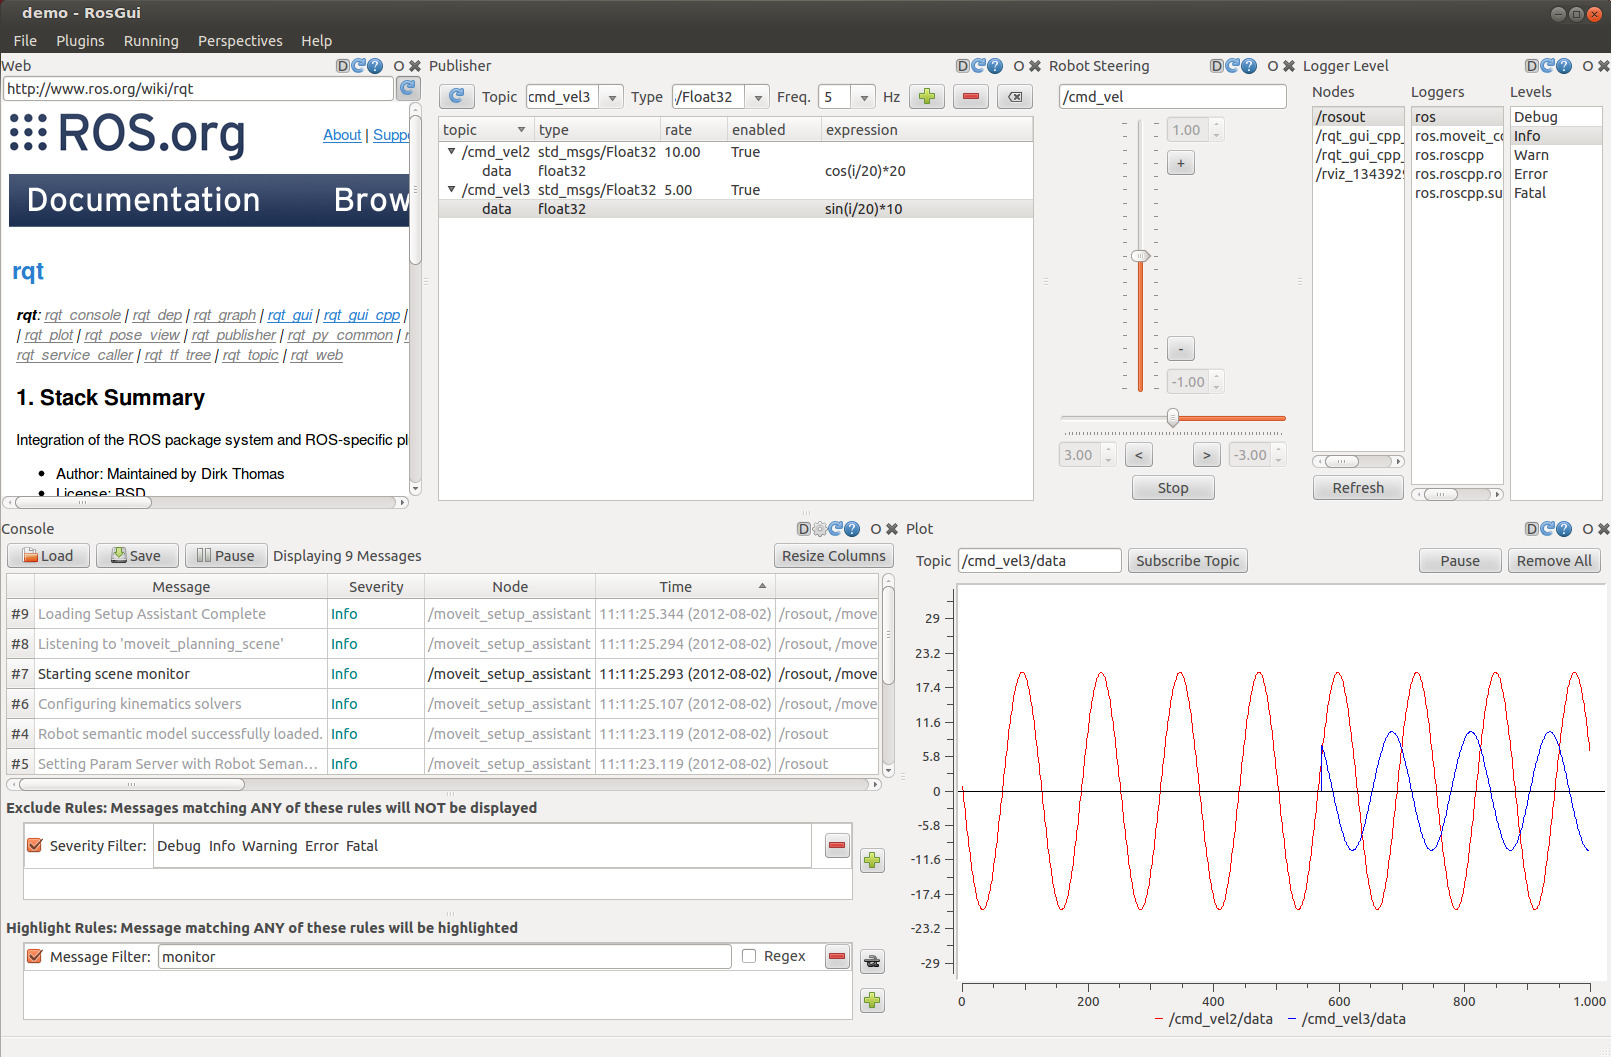
\includegraphics[width=\textwidth]{Figuras/2_revisao/ros_gui.png}
                \caption{Exemplo de ferramentas gráficas existentes no ROS.}
                \label{fig:ros_gui}
            \end{figure}
            
            Essas ferramentas são agrupadas em categorias. Entre elas estão: 
            
            \begin{itemize}
                \item \textbf{Configuração}: reune ferramentas relacionadas a execução e configuração de nós, os \textit{plugins} \textit{rqt\_launch}\footnote{\url{http://wiki.ros.org/rqt_launch}} e \textit{rqt\_reconfigure}\footnote{\url{http://wiki.ros.org/rqt_reconfigure}} são exemplos disso;
                
                \item \textbf{Introspecção}: junta \textit{plugins} para a análise do Grafo de Computação e das dependências entre pacotes;
                
                \item \textbf{\textit{Logging}}: agrupa ferramentas para alternar o nível de \textit{log} nos nós e para filtrar \textit{logs};
                
                \item \textbf{Tópicos}: são reunidas ferramentas diretamente relacionadas tópicos no ROS, como a publicação de mensagens, monitor de tópico e navegador para definições de mensagem;
                
                \item \textbf{Serviços}: cliente de serviços e navegador para definições de serviços, são exemplo de ferramentas relacionadas com serviços;
                
                \item \textbf{Visualização}: agrupa ferramentas que traçam gráficos de dados numéricos no tempo, mostram de imagens publicadas em tópicos e sistemas supervisórios, são exemplos de \textit{plugins} que pertencem a esta categoria \textit{rqt\_image\_view}\footnote{\url{http://wiki.ros.org/rqt_image_view}}, \textit{rqt\_multiplot}\footnote{\url{http://wiki.ros.org/rqt_multiplot}} e \textit{rqt\_rviz}\footnote{\url{http://wiki.ros.org/rqt_rviz}};
                
                \item e muitas outras.
            \end{itemize}
        
    \section{Trabalhos Relacionados} \label{sec:trabalhos_relacionados}
        \citeonline{ref:reis2015alliance} elaborou uma aproximação da arquitetura Alliance dedicada para uma aplicação de patrulhamento